\chapter{Results}
\label{chap:result}

\minitoc 

\section{Reconstruction with SDM}
\label{sec:result-sdm}

\subsection{Reconstruction quality}
\label{sec:result-reconstruction-error}

\begin{figure}
    \centering
    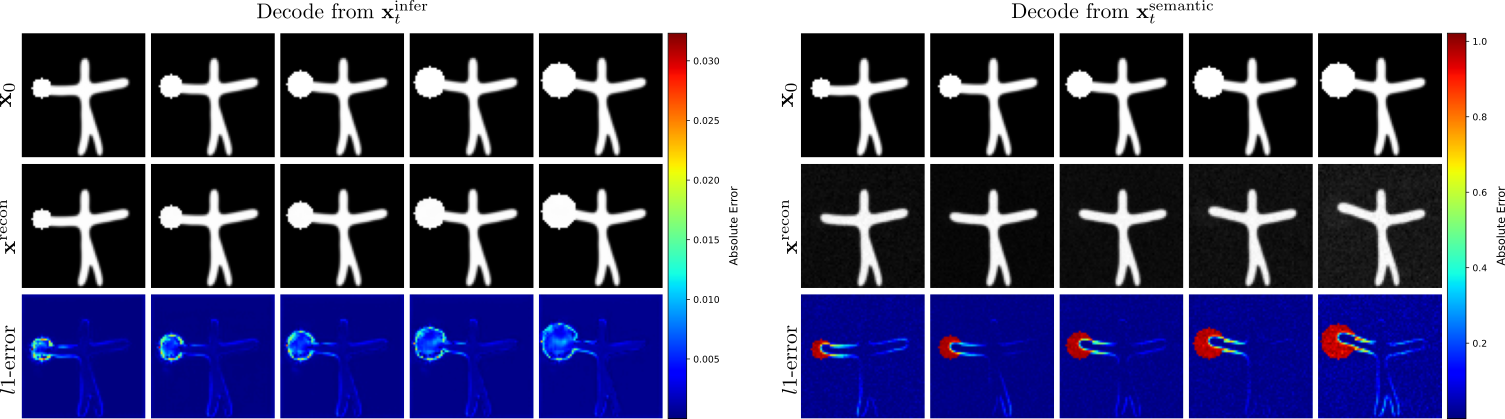
\includegraphics[width=0.75\linewidth]{figures/compare-effect-infer.png}
    \caption[Reconstructions from random noise and from stochastic subcode]{Reconstruction error when decoding from $\rvx_T^{\text{infer}}$ (left) and $\rvx_T^{\text{semantic}}$ (right). From top to bottom: the original image, the reconstructed image and residual error. Note that the color code is not on the same scale for all images.}
    \label{fig:compare-effect-infer}
\end{figure}

\autoref{tab:error-starmen} presents the quantitative results of reconstruction errors for two experiments: denoising from pure random noise and denoising from a stochastic subcode of the input $\rvx$. The term \texttt{semantic} indicates that $\rvx_T$ is obtained by adding random Gaussian noise, whereas \texttt{infer} refers to $\rvx_T$ generated by applying the reversed DDIM process (stochastic encoding) to $\rvx$. All results are evaluated by first noising the image to a noise level of $250$, followed by denoising using the DDIM sampling scheme with 250 denoising steps. We observe that using $\rvx_T^{\text{infer}}$ yields much smaller reconstruction errors and significantly higher similarity metrics. This improvement arises because $\rvx_T^{\text{infer}}$ retains fine-grained details about the input, which are absent in the semantic encoding, and thus better guides the diffusion process toward the true distribution of the original image. For the healthy dataset and subtle anomaly types \texttt{darker\_line} and \texttt{darker\_circle}, we observe extreme cases where MSSIM reaches $100\%$, indicating that perceptually the reconstructed image is indistinguishable from the original to a human observer. On the other hand, this raises a problem of “anomaly preservation", which indicates that the anomaly region is preserved in the reconstructed image. We can see this in the $l_1$-ratio for \texttt{growing\_circle}: it is much higher when denoising from $\rvx_T^{\text{semantic}}$ compared to $\rvx_T^{\text{infer}}$, because the former completely removes the anomaly, whereas the latter preserves it via information encoded in the stochastic subcode. For the case of very subtle anomalies, $l1$-ratio is higher when denoising from $\rvx_T^{\text{infer}}$, this is because the $l_1$-error within the anomaly region is relatively small, which can be attributed to the subtlety of the anomaly. Nevertheless, we can still observe the perceptual effects of anomaly preservation, as well as the qualitative results of different types of reconstruction errors, in \cref{fig:compare-effect-infer}. 

\begin{table}[htbp]
\centering
\caption[Comparison of reconstruction quality]{Comparison of the reconstruction quality of different test datasets. \texttt{\textcolor{blue}{test\_healthy}} refers to healthy dataset, while others correspond to various anomaly types. Dataset name follows format \texttt{<dataset> ($N$)}, where $N$ indicates the number of patients (each patient has 10 longitudinal samples). For all metrics, the mean ± standard deviation across whole dataset are reported. The arrows $\uparrow$ and $\downarrow$ indicate that higher and lower values are favorable, respectively.}
\label{tab:error-starmen}

\begin{subtable}{\textwidth}
    \centering
    \begin{adjustbox}{max width=\textwidth}
    % \resizebox{0.95\textwidth}{!}{%
    \begin{tabular}{lrrrr}
    \toprule
     & \multicolumn{2}{r}{\texttt{\textcolor{blue}{test\_healthy}} (150)} & \multicolumn{2}{r}{\texttt{\textcolor{red}{growing\_circle}} (20)} \\
     & semantic & infer & semantic & infer \\
    \midrule
    $l1 \mathrm{-All}$ (e-3) $\downarrow$ & 12.61 ± 23.94 & 1.04 ± 1.97 & 32.79 ± 125.79 & 0.75 ± 2.07 \\
    $l1 \mathrm{-Anomaly}$ (e-3) $\uparrow$ & - & - & 743.48 ± 372.27 & 6.52 ± 6.44 \\
    $l1 \mathrm{-Healthy}$ (e-3) $\downarrow$ & - & - & 16.44 ± 33.34 & 0.62 ± 1.63 \\
    $l1 \mathrm{-ratio} \uparrow$ & - & - & 45.23 & 10.58 \\
    \cline{1-5}
    $l2 \mathrm{-All}$ (e-3) $\downarrow$ & 0.73 ± 8.26 & 0.00 ± 0.03 & 16.90 ± 118.55 & 0.00 ± 0.08 \\
    $l2 \mathrm{-Anomaly}$ (e-3) $\uparrow$ & - & - & 691.34 ± 388.77 & 0.08 ± 0.45 \\
    $l2 \mathrm{-Healthy}$ (e-3) $\downarrow$ & - & - & 1.38 ± 13.98 & 0.00 ± 0.04 \\
    \cline{1-5}
    $D_{f} \mathrm{-All}$ (e-3) $\downarrow$ & 2.48 ± 2.02 & 0.01 ± 0.01 & 31.50 ± 81.52 & 0.02 ± 0.05 \\
    $D_{f} \mathrm{-Anomaly}$ (e-3) $\uparrow$ & - & - & 306.74 ± 165.98 & 0.10 ± 0.08 \\
    $D_{f} \mathrm{-Healthy}$ (e-3) $\downarrow$ & - & - & 25.17 ± 66.19 & 0.02 ± 0.05 \\
    \cline{1-5}
    SSIM $\uparrow$ & 85.70 ± 5.12 & 99.89 ± 0.02 & 75.00 ± 14.64 & 99.86 ± 0.05 \\
    MSSIM $\uparrow$ & 98.85 ± 0.50 & 100.00 ± 0.00 & 93.76 ± 5.09 & 99.99 ± 0.00 \\
    PSNR $\uparrow$ & 32.66 ± 3.00 & 53.27 ± 1.32 & 21.19 ± 6.57 & 53.19 ± 0.66 \\
    \bottomrule
    \end{tabular}
    \end{adjustbox}
    % }
\label{tab:error-starmen-a}
\caption{Reconstruction metrics for healthy dataset and growing circle anomaly}
\end{subtable}

\vspace{0.5em}

\begin{subtable}{\textwidth}
    \centering
    % \resizebox{0.95\textwidth}{!}{%
    \begin{adjustbox}{max width=\textwidth}
    \begin{tabular}{lrrrr}
    \toprule
     & \multicolumn{2}{r}{\texttt{\textcolor{red}{darker\_line}} (20)} & \multicolumn{2}{r}{\texttt{\textcolor{red}{darker\_circle}} (20)} \\
     & semantic & infer & semantic & infer \\
    \midrule
    $l1 \mathrm{-All}$ (e-3) $\downarrow$ & 14.93 ± 42.74 & 0.47 ± 1.88 & 14.60 ± 37.13 & 0.59 ± 2.09 \\
    $l1 \mathrm{-Anomaly}$ (e-3) $\uparrow$ & 400.49 ± 240.64 & 14.48 ± 10.88 & 385.45 ± 230.77 & 19.93 ± 14.25 \\
    $l1 \mathrm{-Healthy}$ (e-3) $\downarrow$ & 13.06 ± 28.79 & 0.41 ± 1.42 & 13.50 ± 28.58 & 0.53 ± 1.64 \\
    $l1 \mathrm{-ratio} \uparrow$ & 30.66 & 35.64 & 28.56 & 37.65 \\
    \cline{1-5}
    $l2 \mathrm{-All}$ (e-3) $\downarrow$ & 2.05 ± 27.42 & 0.00 ± 0.05 & 1.59 ± 19.48 & 0.00 ± 0.08 \\
    $l2 \mathrm{-Anomaly}$ (e-3) $\uparrow$ & 218.28 ± 216.30 & 0.33 ± 0.46 & 201.81 ± 198.32 & 0.60 ± 0.93 \\
    $l2 \mathrm{-Healthy}$ (e-3) $\downarrow$ & 1.00 ± 17.33 & 0.00 ± 0.03 & 1.00 ± 12.06 & 0.00 ± 0.05 \\
    \cline{1-5}
    $D_{f} \mathrm{-All}$ (e-3) $\downarrow$ & 5.65 ± 9.39 & 0.02 ± 0.05 & 3.94 ± 4.49 & 0.03 ± 0.07 \\
    $D_{f} \mathrm{-Anomaly}$ (e-3) $\uparrow$ & 42.74 ± 22.02 & 0.23 ± 0.07 & 25.94 ± 7.16 & 0.36 ± 0.11 \\
    $D_{f} \mathrm{-Healthy}$ (e-3) $\downarrow$ & 5.47 ± 8.92 & 0.02 ± 0.04 & 3.87 ± 4.32 & 0.03 ± 0.07 \\
    \cline{1-5}
    SSIM $\uparrow$ & 84.27 ± 4.92 & 99.94 ± 0.04 & 84.53 ± 4.91 & 99.92 ± 0.04 \\
    MSSIM $\uparrow$ & 98.30 ± 0.60 & 100.00 ± 0.00 & 98.52 ± 0.48 & 100.00 ± 0.00 \\
    PSNR $\uparrow$ & 27.36 ± 2.02 & 54.36 ± 0.91 & 28.43 ± 1.87 & 53.52 ± 1.40 \\
    \bottomrule
    \end{tabular}
    \end{adjustbox}
    % }
\label{tab:error-starmen-b}
\caption{Reconstruction metrics for darker line and darker circle anomaly}
\end{subtable}
\end{table}

\subsection{Stochastic subcode from diffusion model}
\cref{fig:compare-infer-hist} shows the histogram comparing pixel intensities of $\rvx_T^{\text{infer}}$ and $\rvx_T^{\text{semantic}}$. We observe that, because $\rvx_T^{\text{infer}}$ preserves fine-grained details of the original image, its histogram does not follow a strict Gaussian distribution. This effect is more pronounced for anomalous images. This result is in line with the findings of \cite{DiffAE,lozuponeLDAE2025}, which show that the stochastic subcode from the diffusion model preserves semantic information about the input image. This effect is a result of the DDIM deterministic sampling scheme. As shown in other studies, this characteristic is beneficial not only for reconstruction quality but also for image manipulation. As demonstrated in \cite{lozuponeLDAE2025}, by modifying the stochastic subcode, we can alter the original image while preserving its overall structure and semantic meaning. However, this requires training an additional network (for example, a classifier) to obtain the decision vector used to modify $\rvx_T^{\text{infer}}$. The challenges are: (i) the training dataset contains only healthy images, and (ii) $\rvx_T^{\text{infer}}$ is a spatial representation in $\mathbb{R}^{h \times w}$, which necessitates a patch-based approach or another representation learning network. Without deeper analysis, this presents a challenge in removing subtle anomalies in the context of UAD. We leave the exploration of this direction for future work.

\begin{figure}[h]
    \centering
    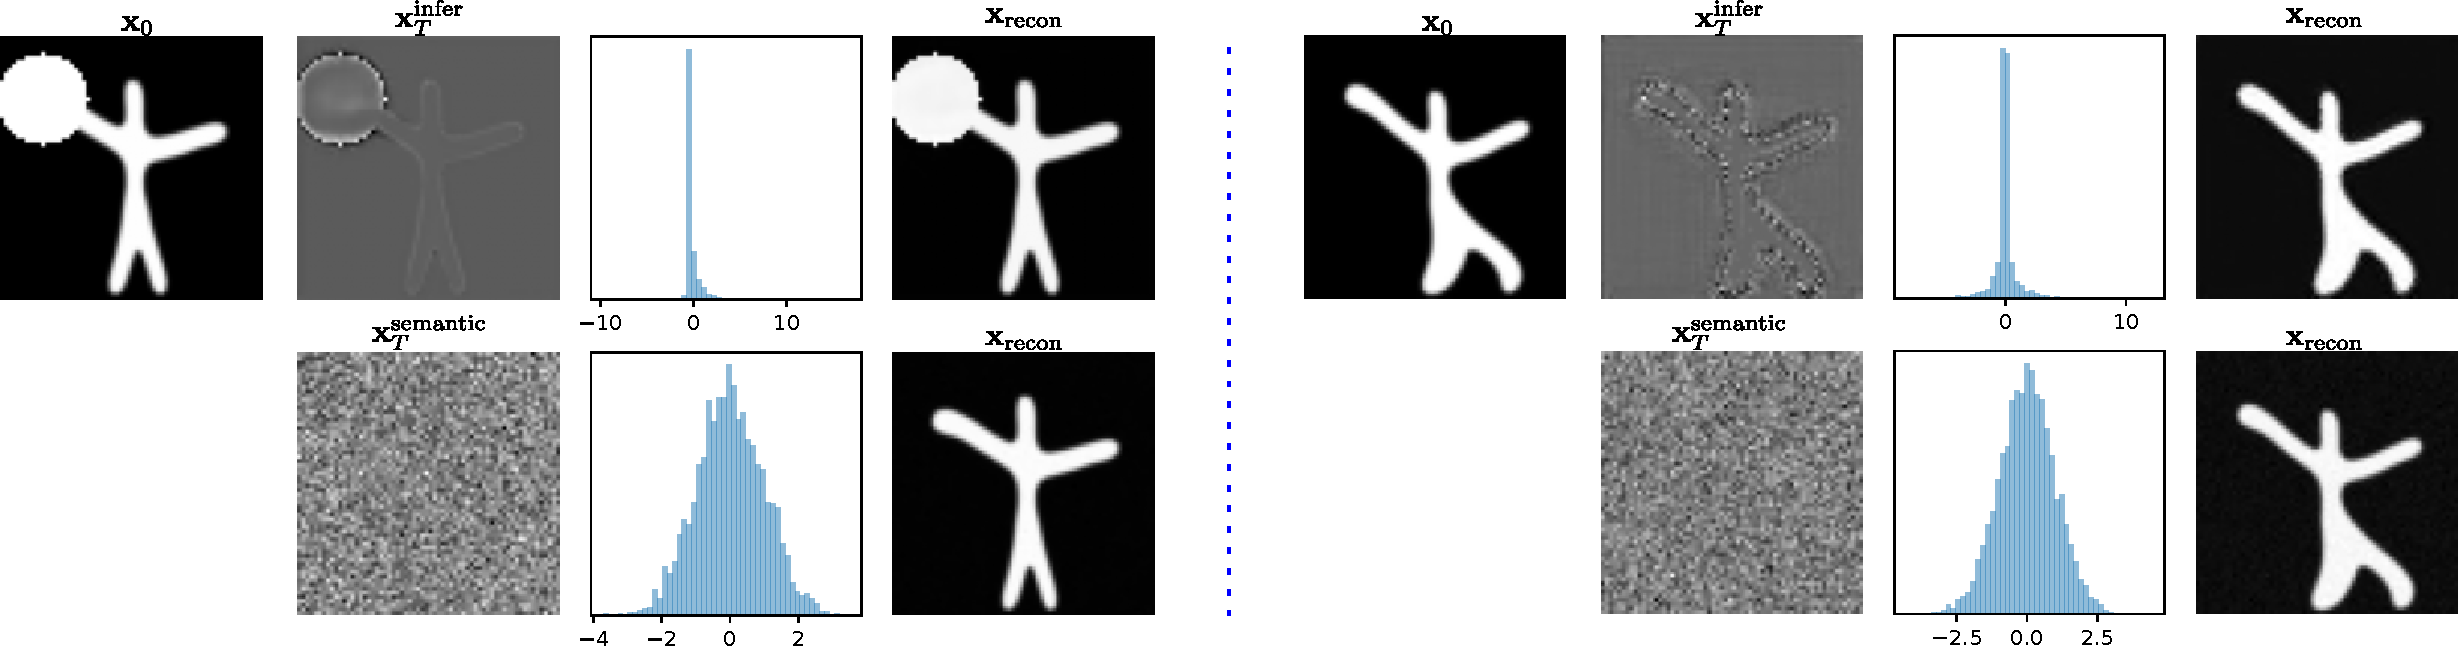
\includegraphics[width=0.75\linewidth]{figures/compare-infer-hist.pdf}
    \caption[Histogram of intensity of random noise and stochastic subcode]{The histogram of intensity of $\rvx_T^{\text{infer}}$ compared to normal noisy $\rvx_T^{\text{semantic}}$, and their corresponding reconstruction. Left: example from anomaly image. Right: example from healthy image.}
    \label{fig:compare-infer-hist}
\end{figure}

\subsection{Effect of noise level on reconstruction errors}
In this section, we investigate the effect of added noise to reconstruction error. \cref{tab:compare-noise-levels} presents the reconstruction errors for different noise levels applied to the input image. We test several noise level from 50 to 1000, with 1000 means that the denoising process starts from pure random Gaussian noise. We observe that lower noise levels (50 and 100) yield better reconstruction quality for healthy anatomy, as indicated by lower $l1$-error and higher SSIM and PSNR values. However, these noise levels result in lower anomaly reconstruction errors, which is undesirable for UAD tasks. Conversely, higher noise levels (750, 800, and 1000) lead to increased anomaly reconstruction errors but also higher reconstruction errors for healthy anatomy. The optimal balance is achieved at a noise level of 250, which provides a good trade-off between accurately reconstructing healthy anatomy and effectively removing anomalies. This result is inline with the \emph{noise paradox} discussed in \cite{autoDDPM}.  

\cref{tab:compare-noise-level-anomalies} provides a detailed breakdown of reconstruction errors for each anomaly type across different noise levels. We observe that the \texttt{growing\_circle} anomaly (large and more noticeable anomalies) type shows the most significant increase in anomaly reconstruction error as the noise level increases, while the \texttt{darker\_line} and \texttt{darker\_circle} (more subtle) anomaly types show more moderate increases. This suggests that the effectiveness of anomaly removal may vary depending on the nature of the anomaly and its contrast with the surrounding healthy tissue. Anomaly with higher intensity needs more noise to be effectively removed, while subtle anomalies require more moderate nosie levels and need more dedicated handling to preserve healthy anatomy.

\begin{table}[h]
    \centering
    \resizebox{1.\textwidth}{!}{
    \begin{tabular}{lrrrrrrrr}
    \toprule
     & \multicolumn{5}{c}{Healthy} & \multicolumn{3}{c}{Anomalies} \\
     \cmidrule(lr){2-6} \cmidrule(lr){7-9}
     & $l$1-error(1e-3)$\downarrow$ & SSIM(\%) $\uparrow$ & MSSIM(\%) $\uparrow$ & PSNR $\uparrow$& LPIPS(1e-3) $\downarrow$ & $l$1-Ano(1e-3) $\uparrow$& $l$1-Healthy(1e-3)$\downarrow$ & $l$1-ratio $\uparrow$\\
    Noise level &  &  &  &  &  &  &  &  \\
    \midrule
    50 & \textbf{10.678} & 84.771 & 98.864 & \textbf{36.908} & 38.093 & 323.192 & \textbf{11.737} & 27.537 \\
    100 & 11.132 & 85.222 & \textbf{98.902} & 35.697 & 35.431 & 508.632 & 12.076 & 42.119 \\
    250 & 12.615 & 85.694 & 98.852 & 32.655 & 32.041 & 653.881 & 13.111 & \textbf{49.873} \\
    400 & 13.704 & \textbf{85.806} & 98.751 & 31.084 & 30.399 & 666.405 & 14.070 & 47.365 \\
    500 & 14.273 & 85.586 & 98.677 & 30.508 & 30.457 & 669.581 & 14.628 & 45.775 \\
    600 & 14.642 & 85.486 & 98.635 & 30.162 & \textbf{30.288} & 671.424 & 14.999 & 44.763 \\
    750 & 15.250 & 84.954 & 98.547 & 29.850 & 31.434 & 672.778 & 15.598 & 43.133 \\
    800 & 15.420 & 84.885 & 98.513 & 29.793 & 31.366 & 673.050 & 15.759 & 42.708 \\
    1000 & 17.953 & 83.505 & 97.989 & 29.539 & 34.377 & \textbf{674.115} & 18.192 & 37.056 \\
    \bottomrule
    \end{tabular}
    }
    \caption[Effects of noise level on reconstruction errors]{The effects of applying different noise levels on reconstruction errors. Arrows $\uparrow$ and $\downarrow$ indicate that higher and lower values are favorable, respectively. The best results are highlighted in \textbf{bold}. Results for the anomalous datasets represent the average over all three types of anomalies.}
    \label{tab:compare-noise-levels}
\end{table}

\begin{table}[h]
    \centering
    \resizebox{1.\textwidth}{!}{
    \begin{tabular}{lrrrrrrrrr}
    \toprule
     & \multicolumn{3}{c}{growing circle} & \multicolumn{3}{c}{darker line} & \multicolumn{3}{c}{darker circle} \\
     \cmidrule(lr){2-4} \cmidrule(lr){5-7} \cmidrule(lr){8-10}
     & $l$1-Ano(1e-3) $\uparrow$& $l$1-Healthy(1e-3)$\downarrow$ & $l$1-ratio $\uparrow$ & $l$1-Ano(1e-3) $\uparrow$& $l$1-Healthy(1e-3)$\downarrow$ & $l$1-ratio $\uparrow$ & $l$1-Ano(1e-3) $\uparrow$& $l$1-Healthy(1e-3)$\downarrow$ & $l$1-ratio $\uparrow$ \\
    Noise level &  &  &  &  &  &  &  &  &  \\
     \midrule
    50 & 313.516 & 18.810 & 16.668 & 352.260 & 12.660 & 27.824 & 349.308 & \textbf{11.849} & 29.480 \\
    100 & 553.121 & 19.249 & 28.735 & 384.994 & \textbf{12.228} & \textbf{31.486} & 372.165 & 11.993 & \textbf{31.031} \\
    250 & 743.802 & 16.359 & 45.467 & 399.816 & 13.063 & 30.608 & 384.890 & 13.706 & 28.081 \\
    400 & 759.369 & \textbf{15.821} & \textbf{47.998} & 403.404 & 13.983 & 28.851 & 388.863 & 15.188 & 25.604 \\
    500 & 763.256 & 15.957 & 47.831 & 404.529 & 14.598 & 27.711 & 389.978 & 16.020 & 24.343 \\
    600 & 765.465 & 16.096 & 47.557 & 405.295 & 14.983 & 27.051 & 390.802 & 16.633 & 23.495 \\
    750 & 767.102 & 16.423 & 46.709 & 405.784 & 15.375 & 26.393 & 391.408 & 17.630 & 22.201 \\
    800 & 767.445 & 16.445 & 46.668 & \textbf{405.840} & 15.404 & 26.346 & 391.492 & 17.997 & 21.754 \\
    1000 & \textbf{768.724} & 17.109 & 44.931 & 405.403 & 16.318 & 24.845 & \textbf{393.398} & 22.926 & 17.159 \\
    \bottomrule
    \end{tabular}
    }
    \caption[Reconstruction errors with different noise levels on anomalous subjects]{Details of reconstruction errors with different noise levels on anomaly datasets. Best results are highlighted in \textbf{bold}}
    \label{tab:compare-noise-level-anomalies}
\end{table}

\section{Unsupervised Anomaly Detection}
In this section, we present the result of anomaly detection using psuedo-healthy image from trained SDM model. All reconstructed images are obtained by denoising from $\rvx_T^{\text{infer}}$ (adding random Gaussian noise to original image). All experiences are done with added noise level of 250, and DDIM sampling is used with 100 denoising steps. 

\begin{figure}
    \centering
    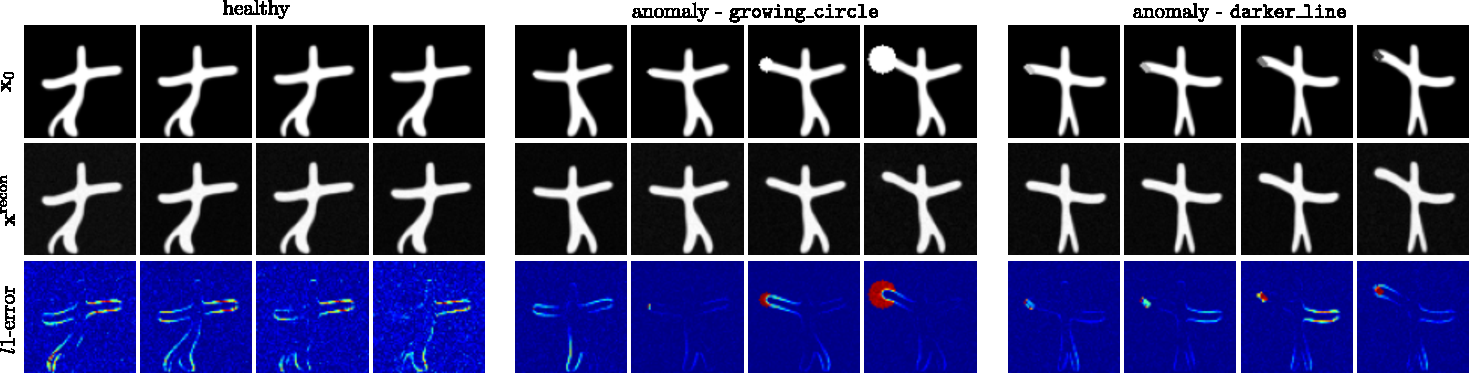
\includegraphics[width=1\linewidth]{figures/ex-recon-error.pdf}
    \caption[Example of $l1$-error for healthy and anomalous subjects]{Example of residual error $l1$-error for healthy and anomaly subjects. From top to bottom: original image, reconstructed image, and residual error. Left: healthy subject. Middle: anomaly subject with \texttt{growing\_circle}. Right: anomaly subject with \texttt{darker\_line}. Note that the color code is not on the same scale for all images.}
    \label{fig:example-recon-error}
\end{figure}

\cref{fig:example-recon-error} shows examples of residual error ($l1$-error) for healthy and anomaly subjects. Visually, the anomaly part can be detected by the high residual error, relatively compared to other parts of the image. However, choosing a proper threshold is proven to be non-trivial, as we can observe high residual error in some healthy parts due to reconstruction quality. This leads to high false positive rate when using simple threshold methods. We can follow some post processing steps from existing literature, such as removing small connected components, but this approach requires prior knowledge about the size of anomalies \cite{behrendt2025cDDPM}. In this work, we target subtle anomaly type for Parkinson disease, and we do not want to make any assumption about the anomaly size. On the other hand, we see that at early stage of disease progression, when the anomaly is very small, residual error is hard to distinguish from other healthy parts. This leads to false negative challenge, which can be more detrimental in clinical screening. \cref{fig:example-seg} shows the results of using naive quantile threshold methods: it generates extremely high false positive rate, for both healthy and anomalous subjects. 

\subsection{Anomaly segmentation with Feature Attention Module}

To address the shortcomings of the pixel residual map, our \ac{FAM} module is designed to attend to the information from the feature distance between the original images and their pseudo-healthy reconstructions. Unlike pixel distance, feature distance focuses more on perceptual differences between two images, highlighting errors only when there is a distortion in the overall image structure. \ac{FAM} learns to ignore minor pixel residuals (reconstruction errors) from our trained FE network $\Phi$ (\cref{sec:feature-extractor-network}). 

\begin{figure}[h]
    \centering
    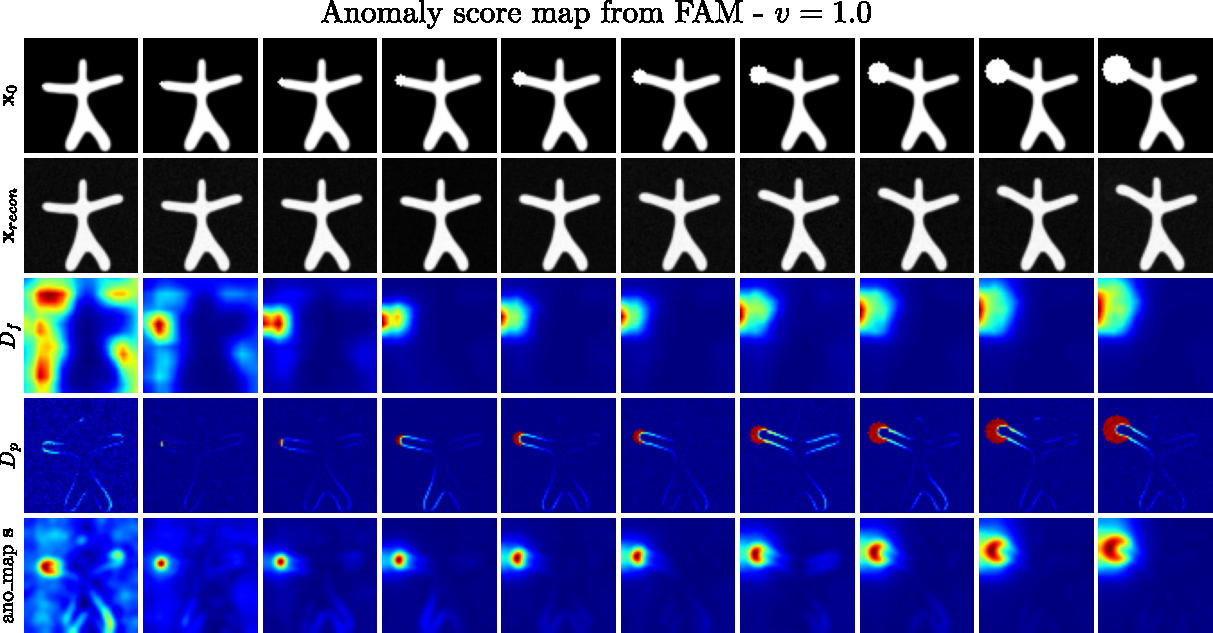
\includegraphics[width=0.75\linewidth]{figures/ano-score-map-gcircle.pdf}
    \caption[Anomaly score map from FAM]{Anomaly score map as combination of feature distance and pixel distance. From top to bottom: original image, reconstructed image, pixel distance, feature distance, and anomaly score map as combination of both. The hyperparameter is $v=1$.}
    \label{fig:ano-score-map-gcircle}
\end{figure}

\cref{fig:ano-score-map-gcircle} shows the anomaly score maps from \ac{FAM} as a combination of feature distance $D_f$ and pixel distance $D_p$. The feature distance correctly captures the overall structural changes in the image. By combining $D_f$ and $D_p$, \ac{FAM} reduces reconstruction errors and shifts the focus to regions with high residual and perceptual errors. However, when anomalies are small and subtle (at an earlier stage), we still encounter false negatives—for example, the residual error in the correct region may be relatively small compared to other healthy regions. Note that the color code in \cref{fig:ano-score-map-gcircle} are not on the same scale. At time $l=0$, the red region indicates the highest value in the feature distance map, but the actual feature error there is very small (close to 0), as shown in \cref{fig:hist-fd-id-gcircle}.

\begin{figure}[h]
    \centering
    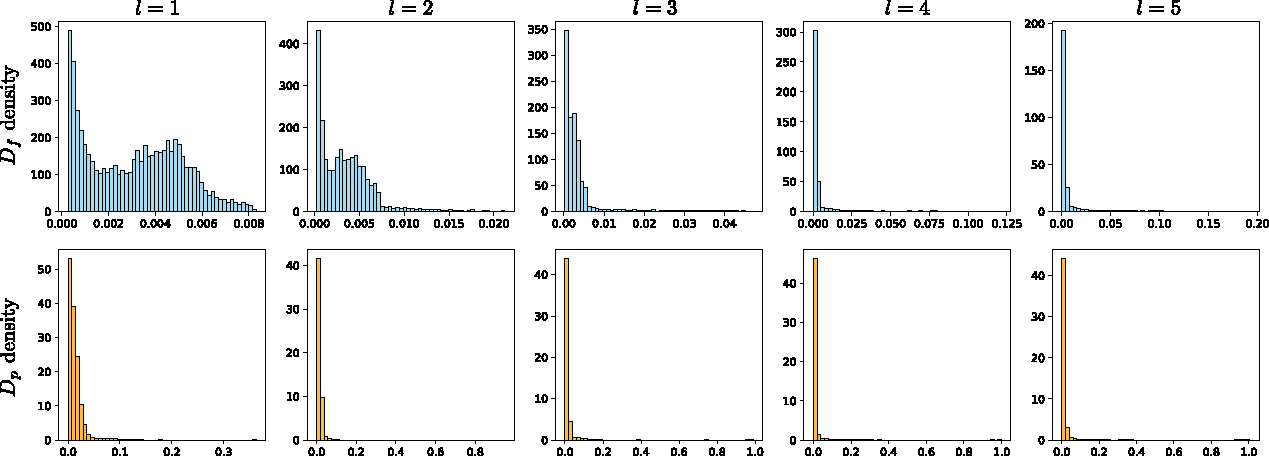
\includegraphics[width=0.75\linewidth]{figures/hist-fd-id-gcircle.pdf}
    \caption[Example of normalized histogram of $D_f$ and $D_p$]{Example of normalized histogram of feature distance $D_f$ (top row) and pixel distance $D_p$ (bottom row) for different time points $l$. }
    \label{fig:hist-fd-id-gcircle}
\end{figure}

\cref{fig:hist-ano-map} shows the effect of using \ac{FAM} on the pixel distance map. For anomalous subjects, the normalized histogram of residual errors is not a reliable indicator for separating anomalous pixels from healthy ones. By using the feature distance, \ac{FAM} spreads out the histogram of residual errors, making it easier to apply automatic thresholding or quantile-based methods to localize anomaly regions.

\begin{figure}[h]
    \centering
    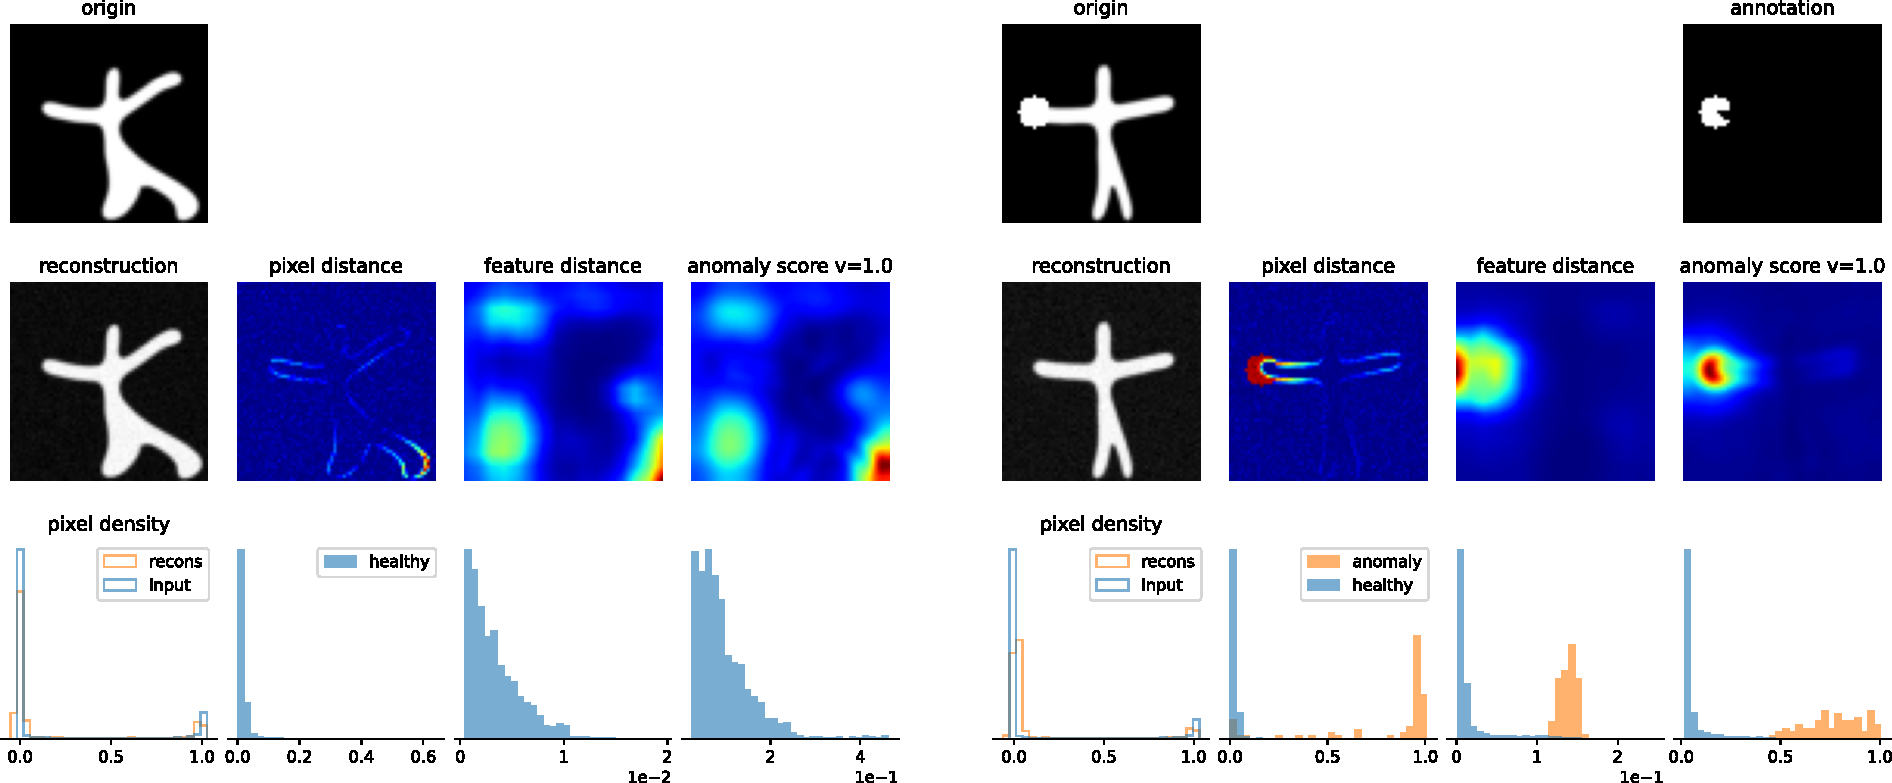
\includegraphics[width=1\linewidth]{figures/hist-ano-map.pdf}
    \caption[Effect of FAM on anomaly score map]{The effect of combination of feature distance and pixel distance. Left: example of healthy image. Right: example of anomaly image. The hyperparameter is $v=1$}
    \label{fig:hist-ano-map}
\end{figure}

\begin{figure}[htbp]
    \centering
    \begin{subfigure}{0.75\textwidth}
        \centering
        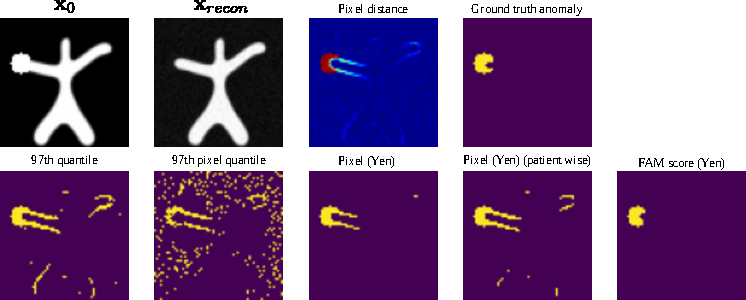
\includegraphics[width=1.0\linewidth]{figures/compare-pix-seg-gcircle.pdf}
        \caption{Anomaly subject.}
        \label{fig:example-seg-gcircle}
    \end{subfigure}
    \hfill
    \begin{subfigure}{0.75\textwidth}
        \centering
        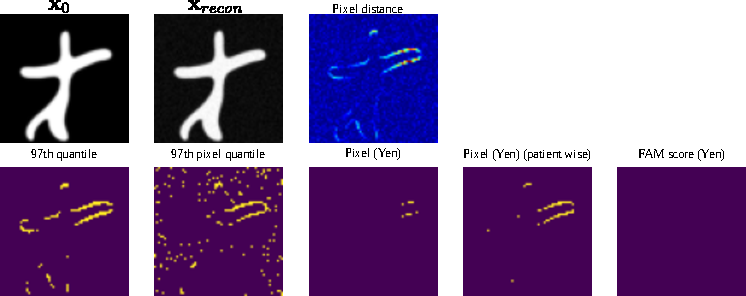
\includegraphics[width=1.0\linewidth]{figures/compare-pix-seg-healthy.pdf}
        \caption{Healthy subject.}
        \label{fig:example-seg-healthy}
    \end{subfigure}
    \hfill
    \begin{subfigure}{0.75\textwidth}
    \centering
    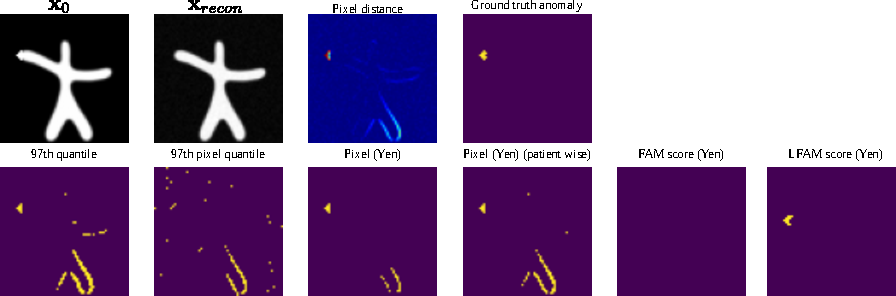
\includegraphics[width=1.0\linewidth]{figures/compare-pix-seg-healthy-false-neg.pdf}
    \caption{Anomaly subject (subtle).}
    \label{fig:example-seg-gcircle-false-neg}
\end{subfigure}
    \caption[Example of anomaly segmentation with different methods]{Example of anomaly segmentation using different methods. \cref{fig:example-seg-gcircle} and \cref{fig:example-seg-gcircle-false-neg} show examples of anomaly subjects, while \cref{fig:example-seg-healthy} shows an example of a healthy subject. The first row: original image, reconstructed image, residual error, and ground truth anomaly segmentation (if any). The second row: segmentation using image-wise 97\% quantile, pixel-wise 97\% quantile, dataset-wise Yen thresholding, patient-wise Yen thresholding, and anomaly score map with \ac{FAM}.}
    \label{fig:example-seg}
\end{figure}

\cref{tab:dice-methods} reports the quantitative results of mDICE scores for different thresholding methods. For the healthy dataset, we also report the false positive percentage (FP\%), i.e., the proportion of the image area incorrectly marked as anomalous. Pixel-quantile methods compute the quantile for each pixel individually, while quantile methods compute it over the whole image (dataset-wise). Yen method applies Yen automatic threshold technique to the pixel distance map $D_p$. \ac{FAM} calculates the anomaly score map by combining feature distance and pixel distance. Quantile methods are applied to the entire test dataset. For the Yen and \ac{FAM} methods, results are reported for both dataset-wise and patient-wise thresholds. The dataset-wise method computes a single threshold value for the whole test dataset (including both healthy and anomalous images). The patient-wise method computes one threshold per patient, considering all observations for that patient (10 observations per patient).

We observe that the classic quantile methods perform poorly in terms of both false positive rates and mDICE scores. The Yen method achieves strong anomaly segmentation performance, attaining some of the highest mDICE scores, except for the \texttt{growing\_circle} anomaly type, where the \ac{FAM} method achieves higher segmentation quality. Moreover, \ac{FAM} yields the best results in terms of minimizing the false positive rate in healthy regions. The result indicates that Yen method has the best overall mDICE score of $69\%$ only if we use the whole dataset to calculate threshold, which increase almost 10\% compared to patient-wise result of $58\%$. We see similar results for \ac{FAM} method, where all mDICE score is higher when the threshold is calculated dataset-wise. This is expected, as having more data provides better information to separate healthy and anomalous pixels. On the other hand, FP is best with patient-wise method. 

\cref{fig:example-seg} displays examples of anomaly localization results for different methods. It is clear that the quantile methods perform poorly, as they fail to disentangle anomaly errors from model reconstruction errors. For healthy subjects, \ac{FAM} outperforms the Yen method in minimizing false positive segmentations.

\begin{table}[htbp]
    \centering
    \resizebox{1.\textwidth}{!}{
    \begin{tabular}{lrrrrrr}
    \toprule
    & & \multicolumn{1}{c}{Healthy} & \multicolumn{4}{c}{Anomaly} \\
    \cmidrule(lr){3-3} \cmidrule(lr){4-7} 
     & &  & growing circle & darker circle & darker line & Total \\
    \multicolumn{2}{c}{Methods} & FP (\%) $\downarrow$ & mDICE\% $\uparrow$ & mDICE\% $\uparrow$ & mDICE\% $\uparrow$ & mDICE\% $\uparrow$ \\
    \midrule
    \multirow{5}{*}{Pixel quantile} & q90.0 & 9.081 & 16.526 & 6.477 & 11.751 & 11.585 \\
                                    & q92.5 & 6.702 & 19.513 & 7.572 & 14.354 & 13.813 \\
                                    & q95.0 & 4.310 & 23.718 & 8.039 & 16.960 & 16.239 \\
                                    & q97.5 & 2.041 & 27.565 & 7.193 & 16.743 & 17.167 \\
                                    & q99.0 & 0.734 & 24.889 & 4.551 & 10.016 & 13.152 \\
    \midrule
    \multirow{5}{*}{Quantile}      & q90.0 & 9.152 & 17.125 & 6.663 & 11.592 & 11.793 \\
                                    & q92.5 & 6.768 & 20.953 & 8.592 & 14.577 & 14.707 \\
                                    & q95.0 & 4.435 & 28.061 & 12.165 & 19.784 & 20.004 \\
                                    & q97.5 & 2.122 & 42.638 & 22.375 & 33.193 & 32.736 \\
                                    & q99.0 & 0.684 & 60.276 & 44.588 & 57.832 & 54.232 \\
    \midrule
    \multirow{2}{*}{Pixel score (Yen)} & dataset wise       & 0.192 & \textbf{76.867} & 59.600 & 70.683 & \textbf{69.050} \\
                                    & patient wise & 1.645 & 47.369 & 58.500 & \textbf{70.872} & 58.914 \\
    \midrule
    \multirow{2}{*}{\shortstack{Anomaly score map \\ FAM}} & dataset wise      & 0.204 & 60.531 & \textbf{65.254} & 62.455 & 62.747 \\
                                        & patient wise & \textbf{0.059} & 57.782 & 49.798 & 44.877 & 50.819 \\
    \bottomrule
    \end{tabular}
    }
    \caption[FP\% and DICE\% for different method]{DICE scores for the anomaly segmentation task, reported for different methods. For anomaly subjects, \texttt{Total} is the average of mDICE scores for all anomaly types. Best results are highlighted in \textbf{bold}.}
    \label{tab:dice-methods}
\end{table}

Notably, one drawback of applying thresholding techniques dataset-wise is that the results strongly depend on the composition of the dataset. Our test dataset comprises 150 healthy subjects and 60 anomalous subjects (20 for each type of anomaly), meaning that approximately 70\% of the samples are healthy. Because healthy images have smaller residual errors, having more healthy references helps to better highlight anomalous regions. \cref{fig:fp-mdice-compare} and \cref{tab:fp-mdice-nb-healthy} illustrate the fluctuations in FP and mDICE scores for different dataset compositions. In particular, we vary the number of healthy subjects while fixing the number of anomalous ones. 

\begin{figure}[htbp]
    \centering
    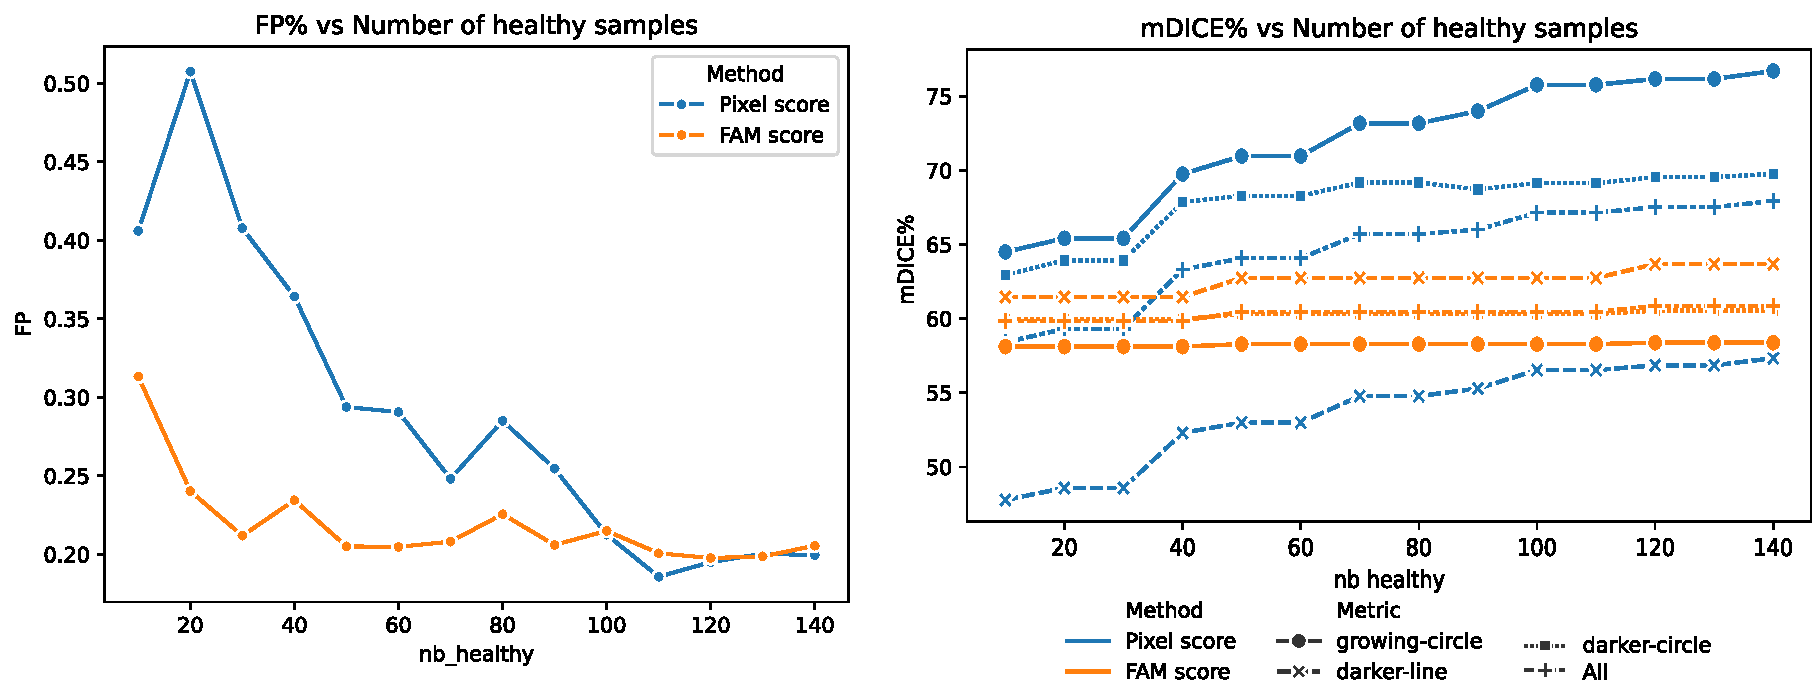
\includegraphics[width=0.9\linewidth]{figures/metric-vs-nb-healthy.pdf}
    \caption[FP(\%) and mDICE(\%) for different unbalanced compositions of dataset]{FP(\%) and mDICE(\%) scores for different unbalanced compositions of the test dataset. Left: FP \% for healthy patients. Right: mDICE \% score for the anomaly segmentation task. The x-axis denotes the number of healthy patients in the dataset, the number of anomalous patients is fixed at 60.}
    \label{fig:fp-mdice-compare}
\end{figure}

As expected, mDICE scores increase as the number of healthy references grows. One interesting observation is that, while the Yen method achieves a higher mDICE score than FAM, FAM demonstrates more stable performance, maintaining consistent scores across different numbers of healthy observations. For false positive rates, FAM also exhibits smaller fluctuations than the Yen method, although we do not see the same consistency as for mDICE.

\begin{table}[htbp]
    \centering
    \resizebox{\textwidth}{!}{%
    \begin{tabular}{lrrrrrrrrrr}
    \toprule
     & \multicolumn{5}{c}{Pixel distance (Yen threshold)} & \multicolumn{5}{c}{Feature Attention Module} \\
     % & \multicolumn{1}{c}{healthy} & \multicolumn{4}{c}{anomaly (mDICE\%)} \\
    \cmidrule(lr){2-6} \cmidrule(lr){7-11}
    & healthy & growing-circle & darker-line & darker-circle & All & healthy & growing-circle & darker-line & darker-circle & All \\
    nb healthy & FP(\%) \textdownarrow & mDICE\% \textuparrow & mDICE\% \textuparrow & mDICE\% \textuparrow & mDICE\% \textuparrow & mDICE\% \textuparrow & mDICE\% \textuparrow & mDICE\% \textuparrow & mDICE\% \textuparrow & mDICE\% \textuparrow \\
    \midrule
    10 & 0.401 & 65.986 & 51.072 & 64.600 & 60.553 & 0.240 & 60.068 & 61.929 & 61.460 & 61.152 \\
    20 & 0.379 & 66.804 & 51.798 & 65.485 & 61.362 & 0.213 & 60.068 & 61.929 & 61.460 & 61.152 \\
    30 & 0.415 & 68.433 & 53.291 & 67.230 & 62.985 & 0.247 & 60.298 & 63.275 & 61.945 & 61.839 \\
    40 & 0.331 & 68.433 & 53.291 & 67.230 & 62.985 & 0.178 & 60.298 & 63.275 & 61.945 & 61.839 \\
    50 & 0.268 & 70.670 & 55.110 & 68.992 & 64.924 & 0.186 & 60.445 & 64.423 & 62.263 & 62.377 \\
    60 & 0.348 & 71.752 & 55.728 & 69.356 & 65.612 & 0.209 & 60.445 & 64.423 & 62.263 & 62.377 \\
    70 & 0.253 & 71.752 & 55.728 & 69.356 & 65.612 & 0.171 & 60.445 & 64.423 & 62.263 & 62.377 \\
    80 & 0.241 & 74.453 & 57.774 & 69.748 & 67.325 & 0.220 & 60.445 & 64.423 & 62.263 & 62.377 \\
    90 & 0.244 & 75.114 & 58.066 & 69.651 & 67.611 & 0.211 & 60.445 & 64.423 & 62.263 & 62.377 \\
    100 & 0.218 & 75.247 & 58.504 & 69.803 & 67.851 & 0.204 & 60.445 & 64.423 & 62.263 & 62.377 \\
    110 & 0.204 & 76.033 & 58.883 & 70.128 & 68.348 & 0.194 & 60.531 & 65.254 & 62.455 & 62.747 \\
    120 & 0.210 & 76.386 & 59.171 & 70.480 & 68.679 & 0.203 & 60.531 & 65.254 & 62.455 & 62.747 \\
    130 & 0.200 & 76.386 & 59.171 & 70.480 & 68.679 & 0.211 & 60.531 & 65.254 & 62.455 & 62.747 \\
    140 & 0.197 & 76.867 & 59.600 & 70.683 & 69.050 & 0.201 & 60.531 & 65.254 & 62.455 & 62.747 \\
    \bottomrule
    \end{tabular}%
    }
    \caption[FP\% and DICE\% for different compositions of test dataset]{FP(\%) and mDICE(\%) results for different numbers of healthy patients in the test dataset. The number of anomaly patients is fixed at 60. The left part of the table shows results using Yen threshold on pixel distance, while the right part shows results using the Feature Attention Module (FAM).}
    \label{tab:fp-mdice-nb-healthy}
\end{table}

In a real case scenario, we do not know the real composition of our test dataset, and ideally we want to improve our method so that it only depends on information per patient, making it more robust for unbalanced dataset. Also, FAM mainly solves the problem of false positive, but for real anomaly detection its performance is still inferior to normal automatic Yen threshold method. \cref{fig:example-seg-gcircle-false-neg} shows 1 example where FAM fails to detect subtle anomaly, while Yen method can detect the anomaly but also include other healthy regions. In the next section, we present our result for anomaly segmentation with our proposed Longitudinal Attention Fusion Module. 

\subsection{Anomaly segmentation with Longitudinal Attention Fusion Module}
By fussing the information from multiple time points, \ac{LAFM} aims to improve the accuracy of anomaly detection, both reducing false positives (anomalies that do not persist over time) and false negatives (use anomalies that are detected from future time points to help detect subtle anomalies at earlier time points).

\begin{table}[]
    \centering
    % \resizebox{1.\textwidth}{!}{%
    \begin{adjustbox}{max width=\textwidth}
    \begin{tabular}{lrrrrr}
    \toprule
     & \multicolumn{1}{c}{Healthy} & \multicolumn{4}{c}{Anomalies} \\
     \cmidrule(lr){2-2} \cmidrule(lr){3-6} 
    & healthy & growing circle & darker circle & darker line & All \\
    methods & FP(\%) \textdownarrow & mDICE\% \textuparrow & mDICE\% \textuparrow & mDICE\% \textuparrow & mDICE\% \textuparrow \\
    \midrule
    Pixel score (dataset wise) & 0.192 & 76.867 & 59.600 & 70.683 & 69.050 \\
    Pixel score (patient wise) & 1.645 & 47.369 & 58.500 & 70.872 & 58.914 \\
    \midrule
    FAM (dataset wise) & 0.204 & 60.531 & 65.254 & 62.455 & 62.747 \\
    FAM (patient wise) & \textbf{0.059} & 57.782 & 49.798 & 44.877 & 50.819 \\
    \midrule
    LAFM ($\sigma=0.0$) & 0.169 & 84.790 & 81.665 & 86.924 & 84.460 \\
    LAFM ($\sigma=0.5$) & 0.198 & 82.441 & \textbf{82.784} & \textbf{87.950} & 84.391 \\
    LAFM ($\sigma=1.0$) & 0.191 & 82.893 & 81.926 & 87.891 & 84.237 \\
    LAFM ($\sigma=1.5$) & 0.178 & 83.604 & 82.682 & 87.909 & 84.731 \\
    LAFM ($\sigma=2.0$) & 0.207 & 85.540 & 81.997 & 87.634 & 85.057 \\
    LAFM ($\sigma=2.5$) & 0.183 & \textbf{86.069} & 81.981 & 87.352 & \textbf{85.134} \\
    LAFM ($\sigma=3.0$) & 0.184 & 85.995 & 81.779 & 87.304 & 85.026 \\
    LAFM ($\sigma=3.5$) & 0.198 & 85.890 & 81.648 & 86.929 & 84.823 \\
    LAFM ($\sigma=4.0$) & 0.194 & 85.762 & 81.826 & 86.893 & 84.827 \\
    LAFM ($\sigma=4.5$) & 0.183 & 85.783 & 81.683 & 86.779 & 84.748 \\
    \bottomrule
    \end{tabular}
    \end{adjustbox}
    %}
    \caption[FP\% and DICE\% for different method - with LAFM]{mDICE and FP scores for different anomaly segmentation methods. The best results are highlighted in \textbf{bold}.}
    \label{tab:dice-lafm}
\end{table}

\cref{tab:dice-lafm} reports anomaly segmentation metrics using LAFM with different variants of Gaussian smoothing $\sigma$. Here, $\sigma=0$ indicates that time points are weighted equally. As discussed in \cref{sec:method-lafm}, $\sigma$ controls the contribution of anomaly score maps from surrounding time points, depending on their distance from the current target image. The mDICE metric increases to around $86\%$, compared to $62\%$ and $69\%$ for FAM and Yen, respectively. LAFM only underperforms FAM in terms of the FP metric, but its result is still comparable to the Yen method, with an acceptable rate of around $0.19\%$. This highlights the trade off between FP and FN: method that achieves the best FP rate processes the residual error more conservatively at the cost of potentially missing some anomalies. On the other hand, method with higher segmentation accuracy will increase the likelihood of anomalies, which leads to more healthy regions being flagged as anomaly. 

\cref{fig:lafm-seg-gcircle} shows 1 example of anomaly segmentation from LAFM. We see that by using information from other time points, we can refine the anomaly map by adding anomaly regions that persist across time and reducing potential anomalies that do not. This effect is more apparent at earlier stages, for example, in the first two time points.

\begin{figure}[htbp]   
    \centering
    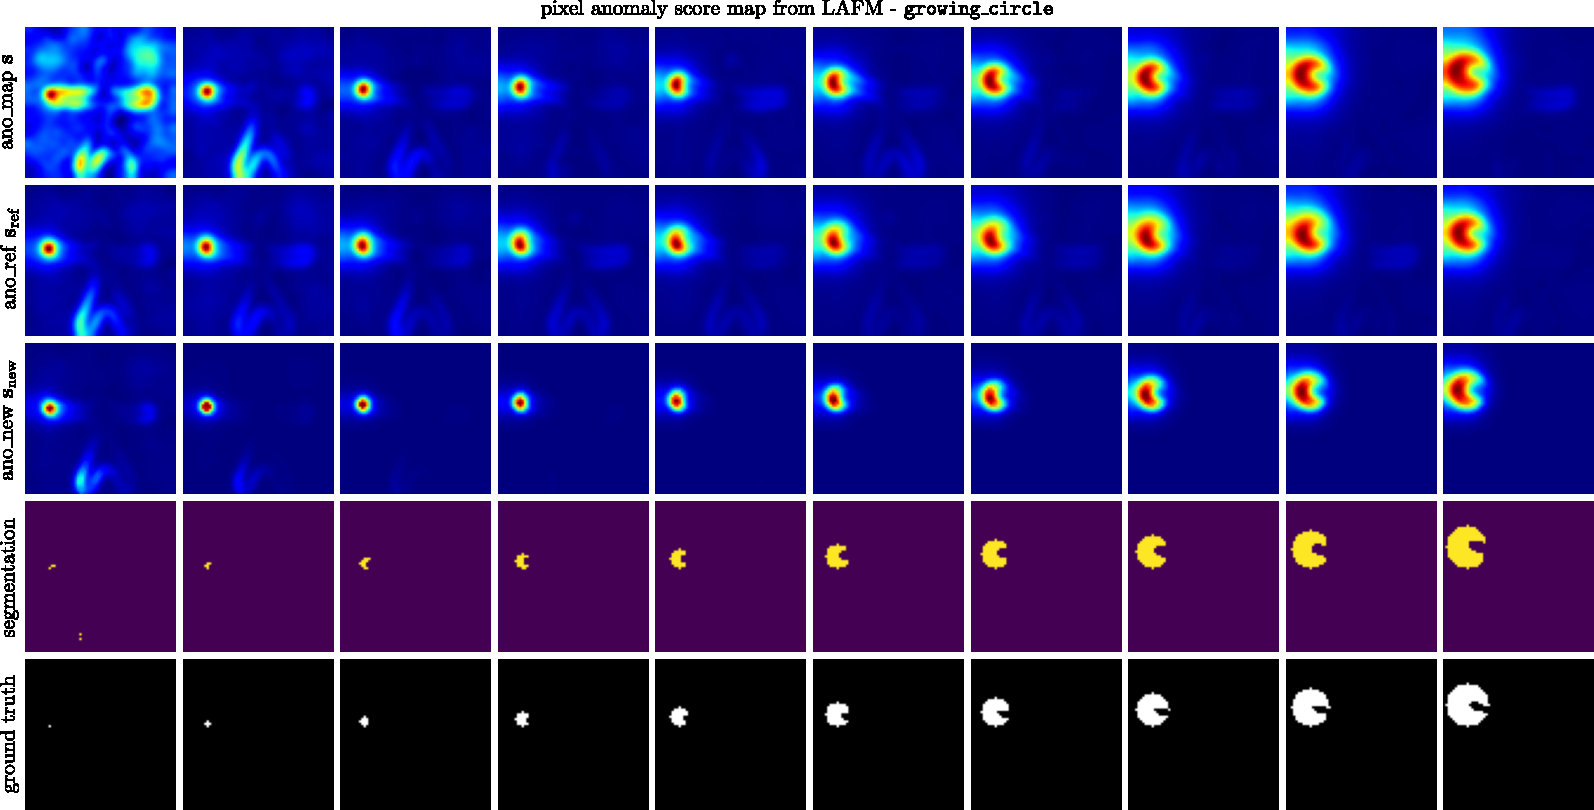
\includegraphics[width=0.75\linewidth]{figures/lafm-seg-gcircle.pdf}
    \caption[Anomaly segmentations from LAFM]{Anomaly segmentation from LAFM. From top to bottom: anomaly map (targeted image), anomaly map references from other time points, updated anomaly map based, anomaly segmentation and ground truth annotation.}
    \label{fig:lafm-seg-gcircle}
\end{figure}

One disadvantage of LAFM is that its performance depends on the number of observations for each patient. The more observations we have, the more additional information we can use to improve the current prediction. \cref{fig:lafm-varying-nbseen} shows the performance of Yen, FAM and LAFM with different numbers of observations (per patient). For each experience, we randomly choose $n$ samples for each patient's longitudinal samples ($\mathrm{max}(n) = 10$). We note that for each $n$, the interval between time points $\Delta_l$ are random. Since the referenced anomaly score maps are weighted by a Gaussian kernel that depends on $\Delta_l$, this randomness can affect the overall performance. To account for this, we run the experience 10 times and reports the average results. 

\begin{figure}[htbp]   
    \centering
    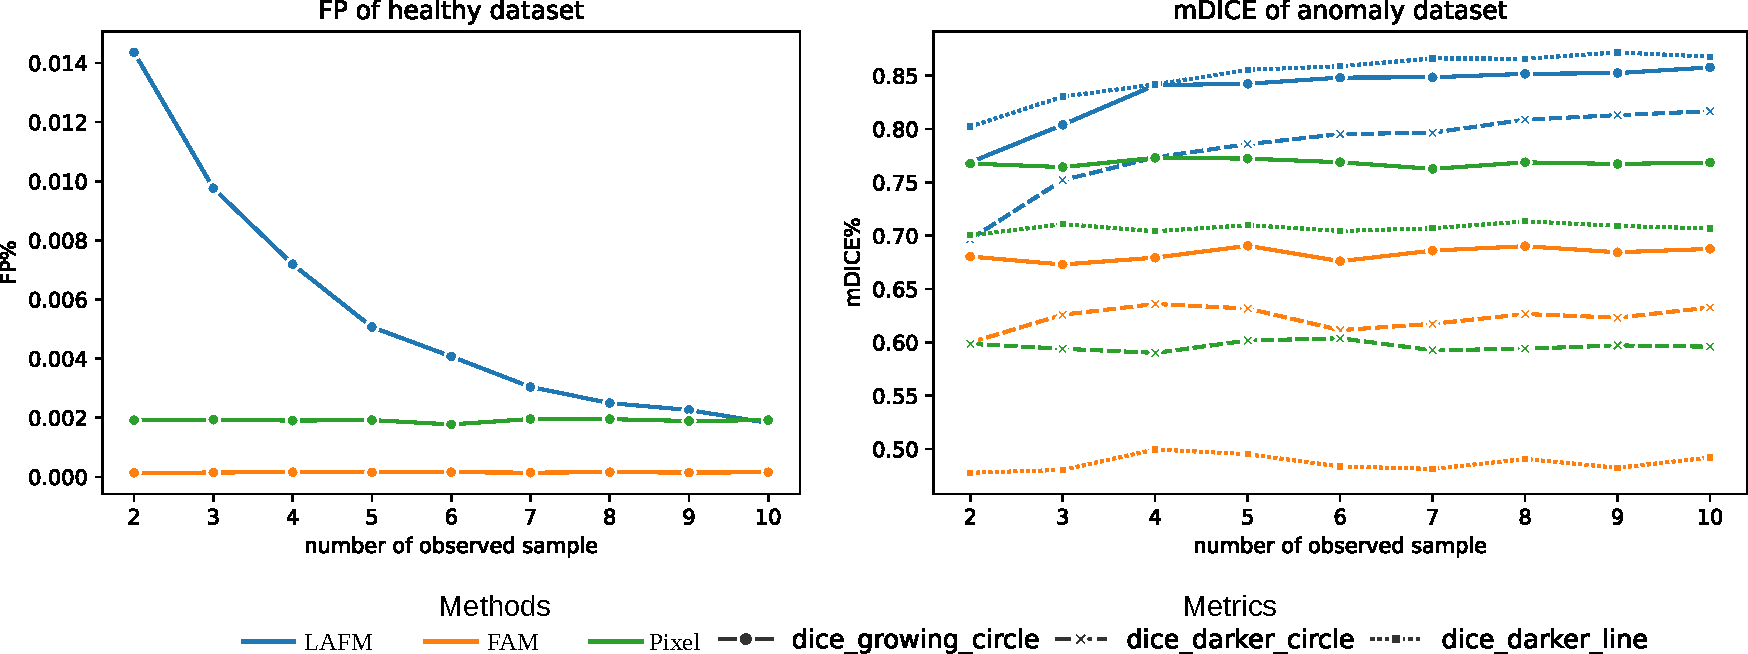
\includegraphics[width=1.0\linewidth]{figures/lafm-varying-nbseen.pdf}
    \caption[FP\% and mDICE\% scores for different numbers of observations]{Comparison of FP\% and mDICE\% scores for different numbers of observed time points. Results for LAFM is calculated with $\sigma=0.5$.}
    \label{fig:lafm-varying-nbseen}
\end{figure}

We see that Yen and FAM have small fluctuations with different number of observations, while LAFM's performance increases as we have more observations. mDICE increases significantly from 2 to 4 observations, and from 4 observations onward, LAFM starts outperforming Yen. On the other hand, FP only reaches stable performance when we have at least 8 observations. This confirms that the strength of LAFM lies in its reliability for anomaly segmentation, rather than in minimizing false positives. 

\cref{fig:lafm-vary-nb} displays the results of pixel anomaly score map with varying number of observations from LAFM. We see that with more observation, we have more referenced information to correct residual errors (e.g. reconstruction error at first time point $l=0$). In the extreme case, in which we only have two observations, and they are far away from each other (time points $l=2$ and $l=9$), the model exhibits negative effect: wrong information (false positive) from the first time point is used as reference for the other. This dilutes the correct anomaly score and reduces the accuracy of segmentation. However, we argue that this cannot be immediately regarded as a defect of the model. By design, LAFM is intended to attend to as much information from longitudinal data as possible. When we have only two observations, it is hard to choose with one  contains the correct information. This holds true specially in real case scenario, when we do not know the ground truth. It can be the case that earlier time point helps correct false positive for later one. 

\begin{figure}[htbp]
    \centering
    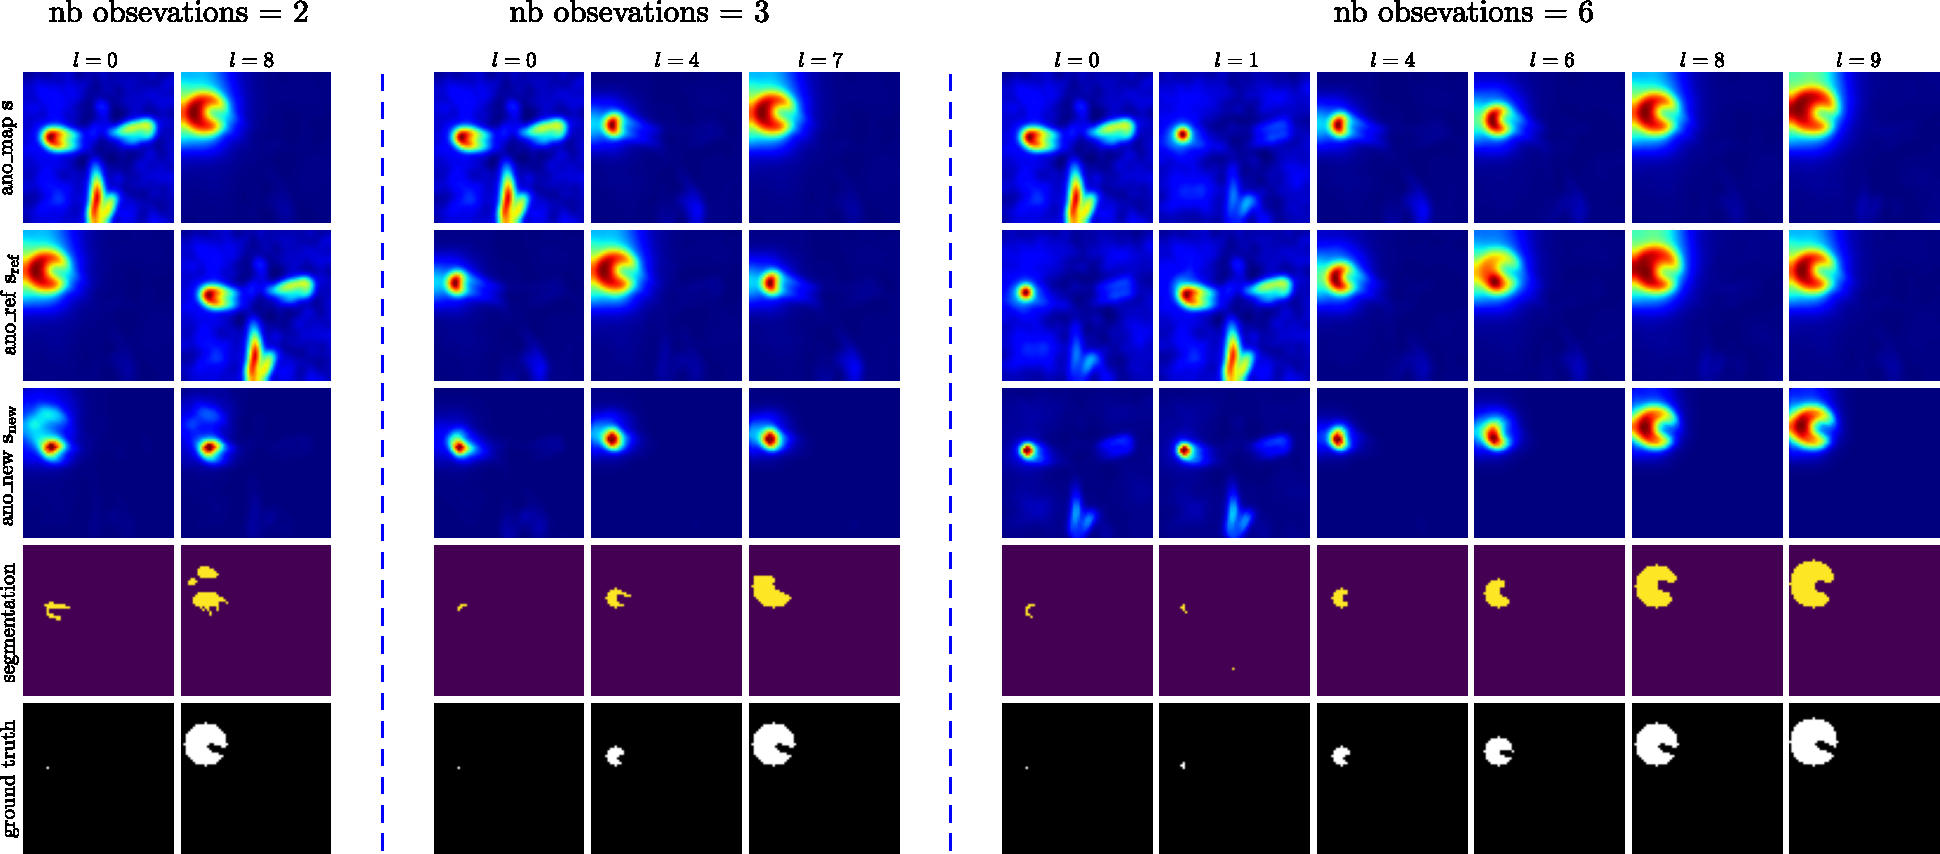
\includegraphics[width=\linewidth]{figures/lafm-vary-nb-fig.pdf}
    \caption{Effect of number of observations on output of LAFM.}
    \label{fig:lafm-vary-nb}   
\end{figure}

\subsection{Image anomaly score}
\label{sec:image-auprc-auroc}

Follow method discussed in \cref{sec:post-process}, we assign image level anomaly score as a summary operator of pixel level anomaly score map. We employ several common strategies, namely: 
\begin{itemize}
    \item \texttt{max}: use the maximum pixel score as image anomaly score. 
    \item \texttt{mean}: assign the average pixel scores as image anomaly score. 
    \item \texttt{mean-top$k$}: calculate the average of top $k$ pixel scores as image anomaly score. 
    \item \texttt{$q$-quantile}: calculate the average of top $q$th percentile pixel scores as image anomaly score. 
\end{itemize}

\cref{tab:auprc-auroc-image} reports the AUPRC and AUROC metrics for different methods and strategies. We apply each strategy to different pixel anomaly score maps that we have obtained so far. Pixel, FAM and LAFM refer to the original pixel residual map $D_p$, pixel anomaly map from FAM and LAFM, respectively. A key observation is that pixel residual error achieves the highest value for both AUROC and AUPRC at 97.5\% and 92.9\% respectively, while our proposed methods FAM only has performance around 86-90\%. We suggest that this may result from the application of several post-processing steps to $D_p$. FAM and LAFM are good for pixel segmentation, but also it neutralizes some information in the pixel residual map. For example, LAFM smooths the pixel anomaly map by concatenating information from other time points, which may reduce the contrast between healthy and anomalous images. 

% , specially FAM and LAFM operate patient wise, while AUPRC and AUROC metrics of image anomaly score is calculated dataset-wise. 
We also see that using max operator remains the best strategy to assign image anomaly score. On the other hand, mean operators have the worst performance, as it average all pixel scores. By doing so, it dilutes the anomaly information because most of our residual errors are small (background pixel). We can observe this effect clearly in mean-top-$k$ and mean-$q$-quantile methods, where the performance increases as we decrease the number of pixels that we consider. On the other hand, we see that LAFM has more stable performance than other methods. Even though mean operators still have lower performance, LAFM remains around 90\% AUROC and 85\%AUPRC, which is better than FAM or Pixel score. \cref{fig:auprc-auroc-curve-pixel} and \cref{fig:auprc-auroc-curve-lafm} show the AUPRC and AUROC curves using pixel distance $D_p$, and LAFM anomaly score, respectively. 

\begin{table}[htbp]
    \centering
    \begin{adjustbox}{max width=\textwidth}
        \begin{tabular}{lrrrrrr}
        \toprule
        & \multicolumn{3}{r}{AUPRC(\%)} & \multicolumn{3}{r}{AUROC(\%)} \\
        \cmidrule(lr){2-4} \cmidrule(lr){5-7}
        & FAM & LAFM & Pixel & FAM & LAFM & Pixel \\
        \midrule
        \texttt{max} & \textit{86.714} & \textit{92.074} & \textbf{92.889} & \textit{90.017} & \textit{96.589} & \textbf{97.509} \\
        \texttt{mean} & 23.558 & 74.778 & 62.905 & 35.604 & 83.692 & 77.458 \\
        \midrule
        \texttt{mean-top50} & 83.040 & 87.680 & 77.815 & 86.630 & 93.547 & 89.823 \\
        \texttt{mean-top100} & 79.827 & 86.380 & 73.208 & 83.723 & 92.484 & 86.521 \\
        \texttt{mean-top150} & 77.073 & 85.752 & 71.114 & 81.295 & 91.872 & 85.002 \\
        \texttt{mean-top200} & 74.347 & 85.266 & 70.011 & 79.067 & 91.422 & 84.242 \\
        \midrule
        \texttt{90.0-quantile} & 62.750 & 83.494 & 68.585 & 70.534 & 90.051 & 83.256 \\
        \texttt{92.5-quantile} & 68.351 & 84.307 & 69.030 & 74.536 & 90.662 & 83.593 \\
        \texttt{95.0-quantile} & 74.068 & 85.215 & 69.939 & 78.842 & 91.379 & 84.192 \\
        \texttt{97.5-quantile} & 79.660 & 86.336 & 73.036 & 83.572 & 92.442 & 86.398 \\
        \texttt{99.0-quantile} & 83.693 & 88.184 & 79.268 & 87.243 & 93.861 & 90.781 \\
        \bottomrule
        \end{tabular}
    \end{adjustbox}
    \caption[AUPRC and AUROC for image anomaly score]{AUPRC and AUROC for image anomaly score. \texttt{mean-top$k$} refers to taking the mean of the top $k$ the highest pixel anomaly scores. \texttt{$q$-quantile} refers to taking the mean of the pixel scores at the $q$th percentile. The best results for AUPRC and AUROC are highlighted in \textbf{bold}, calculated across all methods. Best results for each method are highlighted in \textit{italic}}
    \label{tab:auprc-auroc-image}
\end{table}

\begin{figure}[htbp]
    \centering
    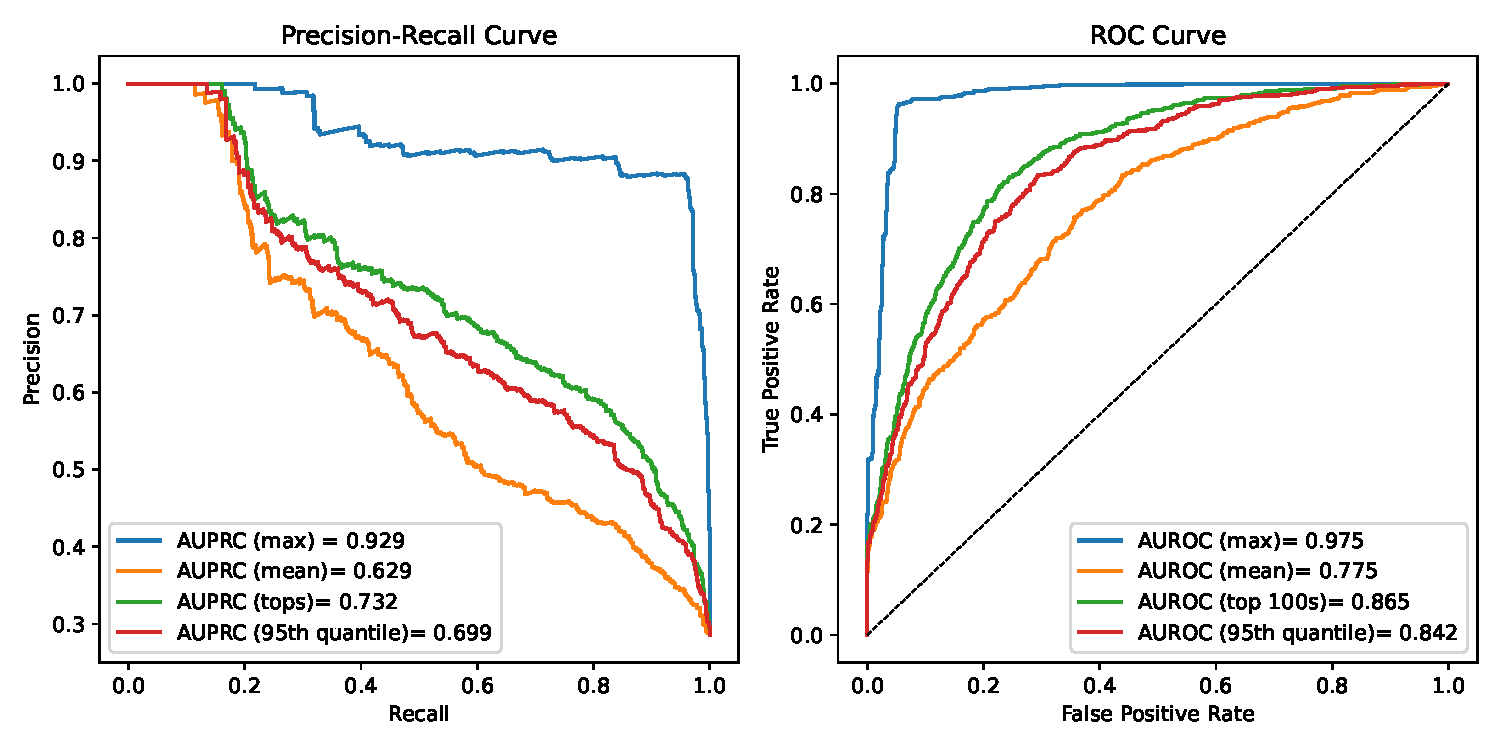
\includegraphics[width=0.8\linewidth]{figures/auprc-auroc-pixel.pdf}
    \caption[AUROC and AUPRC curves for image level score - Pixel distance]{AUROC and AUPRC curves for image anomaly score with different methods, apply to pixel distance $D_p$. Left: AUPRC curves. Right: AUROC curves.}
    \label{fig:auprc-auroc-curve-pixel}
\end{figure}

\begin{figure}[htbp]
    \centering
    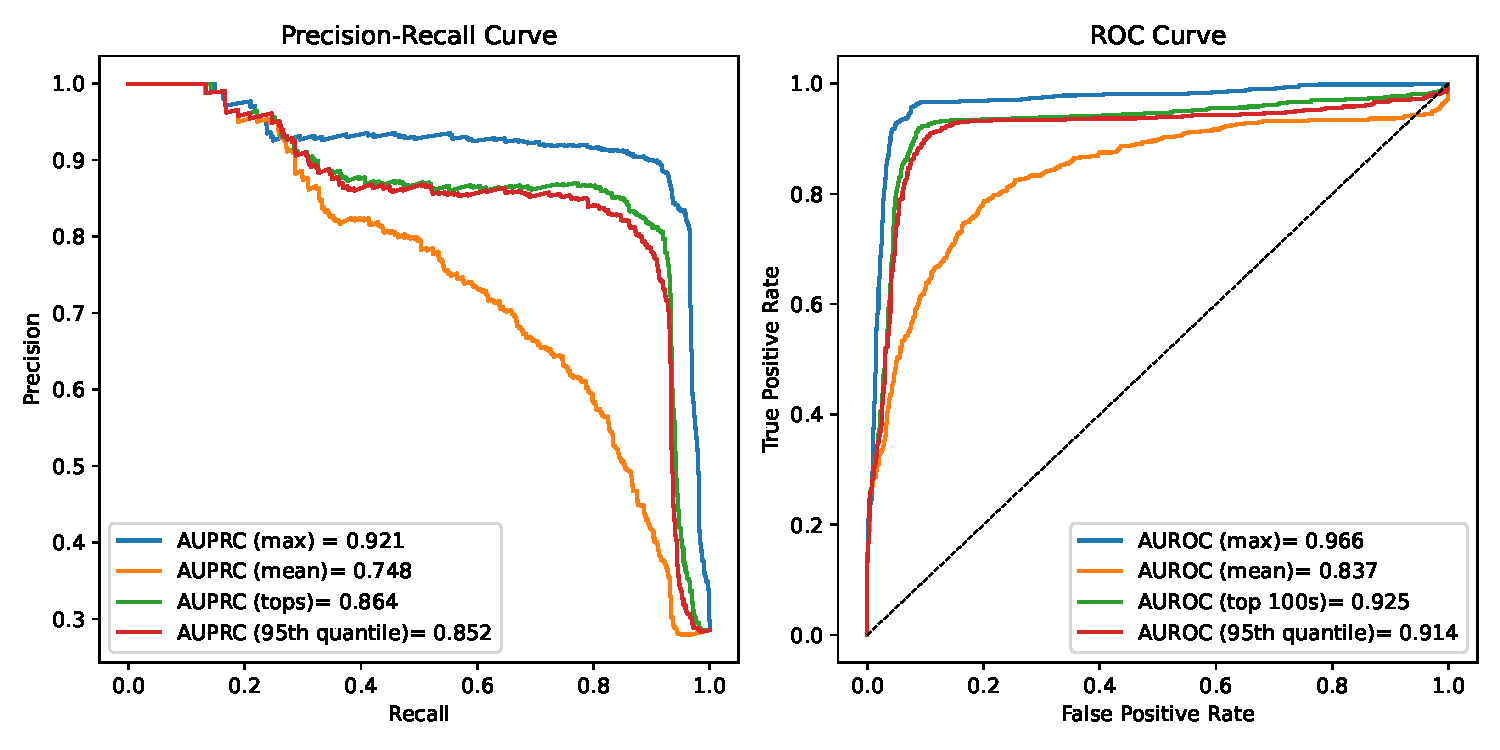
\includegraphics[width=0.8\linewidth]{figures/auprc-auroc-lafm.pdf}
    \caption[AUROC and AUPRC curves for image level score - LAFM score]{AUROC and AUPRC curves for image anomaly score with different methods, apply to LAFM anomaly score. Left: AUPRC curves. Right: AUROC curves.}
    \label{fig:auprc-auroc-curve-lafm}
\end{figure}

